% !TEX program = lualatex
% ECON 201, Worksheet 17: Gains From Trade.
% Compile with LuaLaTeX so the PDF is tagged. Build from the course root:
%   latexmk -lualatex -cd worksheets/worksheet17.tex && latexmk -c -cd worksheets/worksheet17.tex
% Every number here is computed and printed by slides/figures/make_lecture17.py
% (the bread market from the deck under a price cap, CORE Question 8.6
% adapted; the script also draws figures/bread-cap.pdf).
\DocumentMetadata{
  pdfstandard=UA-2,
  pdfversion=2.0,
  lang=en-US,
  tagging=on
}
\documentclass[11pt]{article}

\usepackage[letterpaper, margin=0.75in, top=0.5in, bottom=0.45in]{geometry}
\usepackage{fontspec}
\setmainfont{Fira Sans}
\usepackage{amsmath}
\usepackage{amssymb}
\usepackage{graphicx}
\usepackage{booktabs}
\usepackage{array}
\usepackage{xcolor}
\usepackage{needspace}
\usepackage[most]{tcolorbox}
\definecolor{cream}{HTML}{FDF3EA}
\definecolor{accent}{HTML}{BF5700}
\usepackage{titlesec}
\titleformat{\section}{\large\bfseries\color{accent}}{}{0pt}{}
\titlespacing*{\section}{0pt}{4pt}{2pt}
\usepackage{hyperref}
\hypersetup{pdftitle={ECON 201 Worksheet: Gains From Trade}, pdfauthor={Div Bhagia}, hidelinks}
\pagestyle{empty}
\setlength{\parindent}{0pt}
\setlength{\parskip}{2pt}

% Ruled answer space: n lines. Plain TeX loop; pgffor's \foreach breaks the
% enumerate counter when used inside an item.
\newcount\answerlinecount
\newcommand{\answerlines}[1]{%
  \par\vspace{1pt}\answerlinecount=#1
  \loop\ifnum\answerlinecount>0
    \rule{\linewidth}{0.3pt}\par\vspace{5pt}%
    \advance\answerlinecount by -1
  \repeat
  \vspace{-5pt}}

\begin{document}

{\LARGE\bfseries\color{accent} Worksheet: Gains From Trade}\hfill{\large ECON 201}

% Terms sit on the cream panel, where the brand orange falls below 4.5:1;
% the darker orange keeps WCAG AA contrast (see CLAUDE.md).
\definecolor{accentdark}{HTML}{8F4100}
\newcommand{\term}[1]{\textcolor{accentdark}{\textbf{#1}}}

% Definitions panel list: flush left, compact (see worksheet09).
\newenvironment{deflist}
  {\begin{list}{\textbullet}{%
     \setlength{\leftmargin}{1.1em}\setlength{\labelwidth}{0.7em}%
     \setlength{\labelsep}{0.4em}\setlength{\itemindent}{0pt}%
     \setlength{\listparindent}{0pt}\setlength{\topsep}{2pt}%
     \setlength{\partopsep}{0pt}\setlength{\parsep}{0pt}%
     \setlength{\itemsep}{2pt}}}
  {\end{list}}

\begin{tcolorbox}[colback=cream, colframe=accent, boxrule=0.6pt, arc=2pt,
  left=6pt, right=6pt, top=4pt, bottom=4pt, title=Definitions,
  fonttitle=\bfseries, coltitle=white]
\begin{deflist}
\item \term{Consumer surplus (CS)}: the sum of $\text{WTP} - P$ over every
  unit bought, the area between the demand curve and the price.
\item \term{Producer surplus (PS)}: the sum of $P - \text{MC}$ over every
  unit sold, the area between the price and the supply curve.
\item \term{Total surplus}: consumer surplus plus producer surplus, the
  gains from all the trades in the market. It is largest at the competitive
  equilibrium, where the last unit's WTP equals its MC.
\item \term{Deadweight loss (DWL)}: the surplus lost on trades that would
  create surplus but do not happen.
\end{deflist}
\end{tcolorbox}

\needspace{5\baselineskip}\section{A price cap on bread}

The bakeries in town all sell the same loaf. The graph shows the demand and
supply curves for bread. In equilibrium, 200 loaves a day sell at \$4 each,
and consumer surplus is \$400 and producer surplus \$200.

\begin{center}
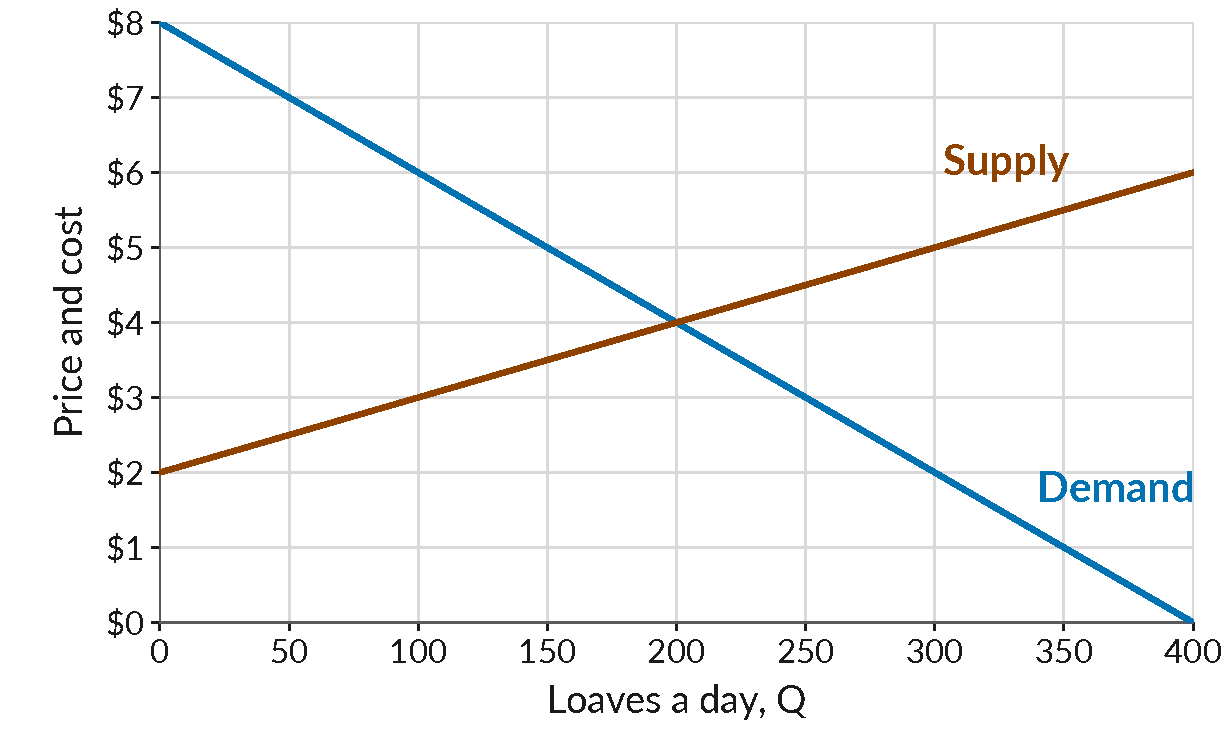
\includegraphics[width=0.6\textwidth, alt={A plotting grid, price and cost on
the vertical axis from 0 to 8 dollars with gridlines every dollar, and loaves
a day on the horizontal axis from 0 to 400 with gridlines every 50 loaves.
The demand curve falls in a straight line from 8 dollars at zero loaves to
zero at 400 loaves. The supply curve rises in a straight line from 2 dollars
at zero loaves to 6 dollars at 400 loaves. They cross at 200 loaves and 4
dollars.}]{figures/bread-cap.pdf}
\end{center}

\vspace{4pt}
1. The city council decides bread is too expensive and caps its price at
\$3 a loaf. At \$3, how many loaves do the bakeries bake? How many do
buyers want? How many loaves sell? Mark the price and the quantity sold on
the graph.
\answerlines{2}

2. Shade the consumer surplus and the producer surplus under the cap, and
compute each.
\answerlines{2}

3. Compared with the equilibrium, who gains from the cap and who loses? By
how much?
\answerlines{2}

4. Shade the deadweight loss and compute it. Which trades does it come from?
\answerlines{2}

5. Is the outcome under the cap Pareto efficient? Explain in one sentence.
\answerlines{2}

\end{document}
